\documentclass{article}
\usepackage[utf8]{inputenc}
\usepackage{hyperref}
\hypersetup{
    colorlinks=true,
    linkcolor=blue,
    filecolor=magenta,      
    urlcolor=cyan,
    breaklinks= true,
}
\usepackage{breakurl}
\usepackage{dirtytalk}
\usepackage{graphicx}
\usepackage{subfig}
\graphicspath{ ./ }


\title{Haskell para la computación gráfica}
\author{Ricardo Rubén González García }
\date{December 2020}

\begin{document}

\maketitle

\section{Propósito}
Demostrar que Haskell puede utilizarse para otras aplicaciones 
aparte de las implementaciones matemáticamente cargadas a las que
se asocia la programación funcional. Con este proyecto se 
intentará aumentar el interés, 
de implementar la programación declarativa para otras áreas más
allá de las más obvias así como dar un pequeño trasfondo teórico a la graficación por computadora

\section{Bibliotecas}
Para poder realizar el modelado 3D a través del código se necesitan 2 cosas:

OpenGL (Open Graphics Library) que es la API que se encargará de realizar todo el modelado. Es la que se encarga de generar polígonos, buffers, matrices, viewport, transformaciones, iluminación, etc.

GLUT (OpenGL Utility Kit) como su nombre lo dice es una extensión de OpenGL. Se encarga de manejar eventos como la creación de ventanas, eventos como modificar el tamaño de la ventana, input del usuario, etc. 

Se usará la versión de OpenGl 2.1 debido a limitantes de hardware.
\section{Preliminares}

Lo primero que debemos aprender es que OpenGL es una máquina de estados. Tiene variables con valores predefinidos que no 
cambiarán a menos que nosotros se lo digamos (como el tamaño de los puntos, las fuentes de luz o qué función es la que se encargará de realizar el dibujado).

Además, es igual de importante saber que todo dentro de OpenGL está operado dentro de matrices y un stack de ellas. 

Por ejemplo, si quisiéramos aplicar una rotación y después una traslación a un punto $p$ situado en $(0,0)$ primero metemos la matriz de desplazamiento, después la de rotación y finalmente dibujamos el objeto.
\begin{table}[h!]
\begin{tabular}{lll}


\cline{1-1} \cline{3-3}
\multicolumn{1}{|l|}{MATRIZ DE DESPLAZAMIENTO}                                                                             & \multicolumn{1}{l|}{$\uparrow$} & \multicolumn{1}{l|}{MATRIZ DE ROTACIÓN}                                                                                   \\ \cline{1-1} \cline{3-3} 
\multicolumn{1}{|l|}{MATRIZ DE ROTACIÓN}                                                                                   & \multicolumn{1}{l|}{$\uparrow$} & \multicolumn{1}{l|}{MATRIZ DE DESPLAZAMIENTO}                                                                             \\ \cline{1-1} \cline{3-3} 
\multicolumn{1}{|l|}{MATRIZ IDENTIDAD}                                                                                     & \multicolumn{1}{l|}{$\uparrow$} & \multicolumn{1}{l|}{MATRIZ IDENTIDAD}                                                                                     \\ \cline{1-1} \cline{3-3} 
\multicolumn{3}{l}{\begin{tabular}[c]{@{}l@{}}Los cambios se van realizando de abajo hacia arriba en el orden en el que van \\ metiendo al stack.\end{tabular}}                                                                                                                          \\ \cline{1-1} \cline{3-3} 
\multicolumn{1}{|l|}{\begin{tabular}[c]{@{}l@{}}Primero realizamos la rotación\\ y después el desplazamiento\end{tabular}} & \multicolumn{1}{l|}{}           & \multicolumn{1}{l|}{\begin{tabular}[c]{@{}l@{}}Primero realizamos el desplazamiento\\ y después la rotación\end{tabular}} \\ \cline{1-1} \cline{3-3} 
\end{tabular}
\end{table}



\subsubsection{Valores importantes de OpenGL y GLUT}
Como ya mencionamos OpenGL es una máquina de estados, por lo que conocer los valores que podemos cambiar resulta de vital importancia para poder comprender el comportamiento de dicha máquina y cómo es que modela un mundo dentro de la aplicación.

\begin{itemize}

    \item \textbf{viewPort}
    
    Es donde inicia y termina la pantalla con la que vemos el mundo generado dentro de la aplicación. La esquina superior isquierda es el $(0,0)$ mientras que la esquina inferior derecha será el valor que nosotros le queramos dar. Por ejemplo: si queremos una pantalla de 700 pixeles por 400, quedaría como $(700,400)$
    
    
    \item \textbf{initialDisplayMode}
    Son valores que necesita saber OpenGL para iniciar y saber cómo es que se comportará el mundo. Si será 2D, 3D, si será con colores o cuántos buffers usará.
    En este proyecto usamos:
    
    \textbf{WithDeptBuffer} porque necesitamos que se vea nuestra escena en 3D y que las cosas que estén detrás de otras se oculten (qué criterio se utiliza para saber qué ocultar se deciden con \textbf{depthFunc}). 
    
    \textbf{depthFunc} compara el valor de profundidad de cada pixel con el que está actualmente en el buffer. En este caso es Less porque si el valor del nuevo pixel es menor (está menos profundo) que el que está en el buffer actual, entonces se pinta. Si fuera Greater, entonces pintaría los píxeles más al fondo por encima de los más cercanos.
    
    \textbf{Doublebuffered} porque queremos tener dos buffers para que no sea vean pantallazos negros en lo que se termina de dibujar algo y se inicia a dibujar la siguiente escena. 
    La idea es que mientras se dibuja un buffer, otro sea el que se muestre y después se inviertan los papeles.
    
    \textbf{RGBMode} porque usaremos colores RGB. Por ejemplo, el (Color3 1 1 (1 :: GLfloat)) es el color blanco, mientras que (Color3 1 0 (0 :: GLfloat)) es el color rojo. Se hace el cast porque la mayoría de las funciones de OpenGL y GLUT no reciben enteros ni floats, sino sus propios tipos. Esto se hace de esta manera para que no dependa del sistema operativo ni de la computadora.
    
    \item \textbf{MatrixMode}
    
    Es la matriz en la que estamos trabajando. 
    Tiene solo 4 valores posibles: GL\_MODELVIEW, GL\_PROJECTION, GL\_TEXTURE y GL\_COLOR. Las que nos importarán para este proyecto serán GL\_PROJECTION y GL\_MODELVIEW
    
    GL\_MODELVIEW es la matriz que nos permite ver la escena y transformar los elementos dentro de la misma (traslaciones, rotaciones, escalas). De ahí su nombre modelado y vista.
    
    GL\_PROJECTION es la matriz que establece qué planos se esconderán, cuáles se mostrarán y de qué tamaño lo harán. Se aplica después de MODELVIEW (como ya dijimos, al trabajar con un stack de matrices el orden es importante, pues stackearlas es lo mismo que ir multiplicándolas)
    
    \item \textbf{Perspectiva}

En OpenGL tenemos varios tipos de perspectiva, pero podemos destacar 2 principalmente: Ortho y Perspective.

\textbf{Ortho} Como su nombre lo indica es una vista ortográfica del \say{mundo} que estamos dibujando; no cambia los tamaños de las cosas independientemente de su distancia del espectador. Sus principales usos es en planos.

\textbf{Perspective} Nos da una vista con perspectiva del \say{mundo}. Aquí los tamaños de las cosas sí variarán dependiendo de la distancia del espectador.

\item \textbf{clearColor}

Es el color con el que se coloreará el fondo de la pantalla

\item \textbf{displayFunc}
Será la función que se llame cada que se quiera refrescar la pantalla.

\item \textbf{Lighting}

La iluminación de OpenGL está basada en 3 partes, la iluminación ambiental, la difusa y la especular. Todas tienen 3 parámetros que son sus valores RGB y qué tanta luz recibe depende del vector normal a los puntos respecto a la fuente de luz.

\item \textbf{shadeModel}
Es qué tipo de sombras tendrá que crear el mundo. Tiene dos valores posibles. FLAT que toma el valor que se computa de un vértice y se lo asigna a toda la cara que se dibuje. SMOOTH hace una interpolación entre los colores de todos los vértices.
\item \textbf{  materialAmbient, materialDiffuse, materialSpecular, materialShininess }

Son valores necesarios para calcular cuánta de qué color va a reflejar la luz y con qué intensidad lo hará. El color resultante que vemos del objeto es una combinación del color de la luz y el del material (por ejemplo, una luz roja y un material que refleje verde será de color café); un material con un valor alto de Shininess será muy brillante y uno con poca se inclinará a los colores mate.

\begin{figure}[h!]
    \centering
    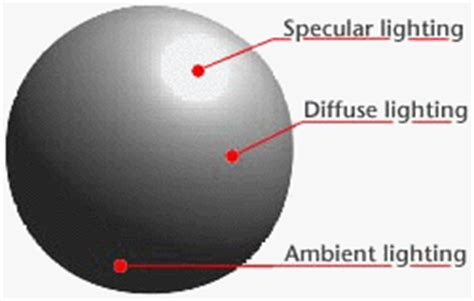
\includegraphics[scale=0.5]{Specular-Diffuse-Ambiental.jpg}

\end{figure}

\item \textbf{keyboardCallback}
Es la función que se encargará de manejar las acciones a realizar cuando el usuario presiona una tecla.
\end{itemize}

\newpage
\subsubsection{El operador \$=}

Este operador cumple dos funciones:
\begin{itemize}
    \item Si tenemos $a$ \$= $b$ y $a$ es IORef, asigna el valor de $b$ en $a$.
    \item Para cambiar los valores de la máquina de estados de OpengGL Así $displayCallback$ \$= $b$ cambia el valor de $displayCallback$ por $b$. displayCallback es la función que se manda a llamar cuando queremos dibujar en la pantalla.
    
\end{itemize}
\subsection{Números aleatorios}
Podemos ver un escenario 3D como una malla de puntos que están unidos entre ellos mediante líneas. Juntando las líneas tenemos caras (usualmente triangulares o a veces cuadrangulares) y al hacer muchas caras muy chiquitas podemos simular una superficie curva. 

Así, dejando fijos los ejes $x$ y $z$ (los límites del mapa) tenemos que calcular una posición $y$ aleatoria para simular las montañas y valles del terreno. Debido a esto, no debe ser solamente aleatoria, porque si no tendríamos el punto (0,100,0) y el (1,-10000,0) juntos y valores tan disparejos no sirven para generar un terreno.

Para solventar este problema se utiliza una función llamada perlinNoise a la que a puntos cercanos les produce números aleatorios cercanos. Así tenemos tanto valores aleatorios como valores que se parezcan entre sí.

\subsection{Generando el terreno}

Una vez que tenemos solventada la altura de los puntos, podemos tomar una tupla de coordinas $(x, z)$ y generar un $Punto3C$ el cual tiene 4 valores: sus tres coordenadas y un color.

Para crear el color podríamos simplemente dejar un color fijo y que sea la combinación del material y de la luz la que se encargue de generar colores distintos, pero decidí también darles valores distintos dependiendo del valor del eje y.

Ya que tenemos una matriz de puntos $(Punto3\ x\ y\ z\ c\ )$ ahora debemos obtener puntos $(Punto3CN\ x\ xn\ y\ yn\ z\ zn\ c\ )$ en el que los valores $(xn,\ yn,\ zn)$ generan el vector normal al punto.

Para esto se crea la función $sacaNormales$ que recibe un punto $p$, obtiene sus vecinos de arriba y de la derecha, los resta para obtener dos vectores y después calcula el producto cruz entre ellos.
\begin{figure}[h!]% 
    \centering
    \subfloat[\centering Se obtienen dos normales por punto en la intersección porque se obtiene la normal de cada cara]{ {\includegraphics[scale = 0.5]{Normals.jpeg} } }%
    \qquad
    \subfloat[\centering Ilustración de cómo obtener el vector normal. Aquí la diferencia es que en lugar de asignarle la misma normal a toda la cara, solo se la asignamos al punto C]{ {\includegraphics[scale = 0.5]{TriangleNormal.jpeg} } }%
    
\end{figure}


\section{Poner la escena}
Lo primero que tenemos que hacer es asignar todos los valores importantes de los que se hablaron en la sección de Preliminares. 

Como reshape se manda a llamar antes de crear la primer ventana, podemos mandar a llamar aquí las funciones para cambiar el viewport, poner la proyección en perspectiva y ajustar la cámara.

Ya que se llama a reshape, inicia a ejecutarse display.

Aquí lo primero que hacemos es limpiar la pantalla del buffer anterior, después hacemos:

\begin{verbatim}
    preservingMatrix $ drawMatrix
\end{verbatim}

¿Qué quiere decir esto? Para empezar usamos el operador \$ porque queremos que se ejecute primero drawMatrix. Ahora, preservingMatrix significa que vamos a meter al stack una matriz nueva, en ella vamos a hacer todos los cambios que se ejecuten en drawMatrix, después de que se termine de ejecutar drawMatrix le hará pop a la matriz, dejando el stack de la forma en que estaba originalmente. Si no hiciéramos esto, todos los cambios que haga drawMatrix se volverían a ejecutar y se irían acumulando dando resultados inesperados.

Dentro de drawMatrix tenemos:

\begin{verbatim}
drawMatrix :: IO ()
drawMatrix = do
  renderPrimitive Quads $ do
      mapM_  drawPointsNormal generateVertexNormalMatrix
\end{verbatim}

Para entender esto un poco mejor, veamos la firma de renderPrimitive. 
\begin{verbatim}
renderPrimitive :: PrimitiveMode -> IO a -> IO a    
\end{verbatim}
PrimitiveMode es un enumerador, son las posibles figuras que puede graficar OpenGL, los valores pueden ser:

\begin{figure}[h!]
    \centering
    \includegraphics[scale = 0.4]{glPrimitives.png}
\end{figure}

En este caso usaremos Quads simplemente por la facilidad para codificarlo, así no tenemos que preocuparnos por cómo ir armando los triángulos y como recorrer sobre todos los puntos para que se dibujen todos correctamente. 

El segundo argumento debe ser algo de tipo IO a, en este caso no queremos regresar nada, simplemente dibujar en la pantalla.

Lo siguiente que se ejecuta es un mapM\_ pero para poder explicarlo, primero tenemos que saber la diferencia entre map y mapM. Supongamos que tenemos una lista de strings y queremos escribirlas en pantalla. Si hacemos

map (putStrLn) lista 

nos daría un error porque estaríamos tratando de devolver una lista de IO () (lo que devuelve putStrLn). Por otro lado 
mapM (putStrLn) lista

Hace exactamente lo que queremos que es escribir cada cadena de la lista en pantalla (es decir va realizando una acción por elemento), pero nos devuelve una lista de () tan larga como la cantidad de cadenas que queramos poner en pantalla.

Para evitar construir esta información que podría ser considerada basura (lo es en este caso, porque no nos interesa lo que devuelve, solo queremos que dibuje. Para otros programas puede que sí nos interese el resultado) y que además nos cuesta tiempo, usamos mapM\_ que siempre regresa m (), en este caso IO ().

Las lista que le pasamos es generateVertexNormal (que está definida en Matrices2 y que genera nuestra matriz de Punto3CN).

La función que le pasamos es drawPointsNormal.
\begin{verbatim}
drawPointsNormal :: Punto3CN -> IO ()
drawPointsNormal p = do
    color $ c1 p
    normal $ Normal3 ( xn p) ( yn p) (sn p)
    vertex $ Vertex3 (x1 p) (y1 p) (s1 p)

    normal $ Normal3 (xn arriba) (yn arriba) (sn arriba)
    vertex $ Vertex3 (x1 arriba) (y1 arriba) (s1 arriba)

    normal $ Normal3 (xn diagonal) (yn diagonal) (sn diagonal)
    vertex $ Vertex3 (x1 diagonal) (y1 diagonal) (s1 diagonal)

    normal $ Normal3 (xn der) (yn der) (sn der)
    vertex $ Vertex3 (x1 der) (y1 der) (s1 der)

    where
      vecindad = agrupa4N p
      arriba = (vecindad !! 1)
      diagonal = (vecindad !! 2)
      der  = (vecindad !! 3)

\end{verbatim}

Como dijimos, usamos Quads y por cómo es la primitiva de OpenGL cada 4 puntos que le pasemos crearemos un nuevo cuadrado. Por lo tanto primero obtenemos los 3 vecinos de cada punto.

Ahora por sintaxis de OpenGL para pintar un vértice primero tenemos que especificar su normal y su color (en el orden que sea). Por lo que aplicamos lo mismo para los 4 vértices. 
Una vez que terminamos de pintar, termina la llamada y volvemos al mainloop de OpenGL cambiando entre buffers.

\section{Teclado}

Para captar las señales del teclado, lo único que verificamos es la tecla que presiona el usuario. WASD se usa para mover la cámara (lo que realmente hacemos es trasladar el terreno hacia los diferentes ejes) e IJKL para mover hacia donde apunta la cámara (que ahora lo que hacemos es trasladar las cosas). Finalmente para salir usamos la tecla ESC o podemos cerrar la ventana. Ambas nos sacan del mainLoop.

\section{Para Correr el proyecto}

Primero se necesita instalar cabal (en caso de que no esté instalado ya) \url{https://www.haskell.org/cabal/index.html#install-upgrade} y ya con cabal instalado:

\begin{verbatim}
    $ cabal install GLUT-2.7.0.15
    $ cabal install hsnoise-0.0.2
\end{verbatim}
Cuando terminen de instalarse:

\begin{verbatim}
    $ ghc --make Main
\end{verbatim}

Lo que creará, entre otras cosas, un ejecutable. Solo resta escribir:

\begin{verbatim}
    $ ./intento
\end{verbatim}
\section{Referencias: }
\sloppy
\begin{enumerate}
    \item \url{https://wiki.haskell.org/OpenGLTutorial1}
    \item  \url{https://hackage.haskell.org/package/OpenGL-3.0.3.0/docs/src/Graphics.Rendering.OpenGL.GL.MatrixComponent.html#MatrixComponent}
    
    \item \url{http://yannesposito.com/Scratch/en/blog/Haskell-OpenGL-Mandelbrot/}
    
    \item \url{https://www.khronos.org/}
    
    \item \url{https://www.haskell.org/hugs/pages/libraries/OpenGL/Graphics-Rendering-OpenGL-GL-CoordTrans.html#v%3ApreservingMatrix}
    
    \item \url{https://hackage.haskell.org/package/OpenGL}
    
    \item \url{https://hackage.haskell.org/package/base-4.12.0.0/docs/System-IO-Unsafe.html}
    
    \item \url{https://stackoverflow.com/questions/28998375/understanding-lighting-in-opengl}
    
    \item \url{https://www.khronos.org/opengl/wiki/GLAPI/glDepthFunc}
    
    \item The Official Guide to Learning OpenGL, Version 1.1
\end{enumerate}
\end{document}

